\documentclass[aspectratio=169]{beamer}
% \documentclass[aspectratio=169,handout]{beamer}

\usetheme[titleformat=regular%
,numbering=fraction% use slide numbers
]{metropolis}
\metroset{%
  progressbar=foot,%
  %background=dark,
  block=fill
}
\only<handout>{\metroset{sectionpage=none}}
\only<handout>{\usecolortheme{dove}}
\usepackage{appendixnumberbeamer} % separate appendix
\usepackage[citestyle=authortitle,sorting=none]{biblatex}
\setbeamerfont{footnote}{size=\tiny}
\addbibresource{mae.bib}

% multimedia in beamer presentations
\usepackage{multimedia}

% adding some better facilities to latex such as proper booleans
\usepackage{etoolbox}

% Unicode math symbols for XeLaTeX
\usepackage{mathrsfs}

% standard math packages
\usepackage{amssymb}
\usepackage{amsthm}
\usepackage{amsmath}
\usepackage{amstext}
\usepackage{mathabx}
\usepackage{stmaryrd}
% math tools for amsmath
\usepackage{mathtools}

\usepackage{proof}

\usepackage{pgfpages}

\usepackage{listings}
\usepackage{xcolor}

% subfigures, subfloats
\usepackage{subcaption}

% for multiinclude
\usepackage{xmpmulti}

% tikz & friends

\usepackage{galois}
\usepackage{tikz}
\usetikzlibrary{fit,calc,shapes,arrows.meta,patterns,backgrounds}
\usetikzlibrary{decorations.pathmorphing}
\usetikzlibrary{cd}
\usetikzlibrary{positioning}
\usepackage[beamer]{hf-tikz}

% for author-title-year citing
\usepackage{xpatch}

\newcommand{\tikzmark}[1]{%
  \tikz[overlay,remember picture,baseline] \node [anchor=base] (#1) {};}

\newenvironment{tightcenter}{%
  \setlength\topsep{0pt}
  \setlength\parskip{0pt}
  \begin{center}
}{%
  \end{center}
}

% new colors
\definecolor{lightblue}{RGB}{217,220,253}
\definecolor{lightred}{RGB}{251,216,218}

\DeclareMathOperator{\pw}{\mathcal{P}} % powerset
\newcommand{\fset}[1]{\mathsf{#1}}
\newcommand{\nats}{\mathbb{N}}
\newcommand{\zahlen}{\mathbb{Z}}
\newcommand{\bools}{\mathbb{B}}
\newcommand{\Set}[1]{\left\{#1\right\}}
\newcommand{\true}{\kw{true}}
\newcommand{\false}{\kw{false}}
\newcommand{\sidenote}[1]{\hfill\quad \textsf{#1}}

\newcommand{\disunion}{+}

% named set
\newcommand{\ns}[1]{\mathit{#1}}
% function
\newcommand{\fn}[1]{\mathrm{#1}}
% "vector of"
\newcommand{\vo}[1]{\overrightarrow{#1}}
% "set of"
\newcommand{\setOf}[1]{\overline{#1}}
% syntactic tag
\newcommand{\sTag}[2]{\textsf{\textbf{#1}}\,#2}
% keyword
\newcommand{\kw}[1]{\texttt{#1}}
% usual suspects
\newcommand{\State}{\ns{State}}
\newcommand{\Value}{\ns{Value}}
\newcommand{\Stmt}{\ns{Stmt}}
\newcommand{\Env}{\ns{Env}}
\newcommand{\Store}{\ns{Store}}
\newcommand{\Kont}{\ns{Kont}}
% syntactic domains
\newcommand{\Exp}{\ns{Exp}}
\newcommand{\Var}{\ns{Var}}
\newcommand{\Addr}{\ns{Addr}}
% put a value to a pointer
\newcommand{\update}{\leftarrow}

% ebnf
\newcommand{\eDEF}{\,::=\;}
\newcommand{\eOR}{\;\vert\;}

\newcommand{\widen}{\nabla}

% \newcommand{\|}{\,\vert\,}

\newcommand{\todo}[1]{\iftoggle{TODO}{\textcolor{red}{TODO: #1}}{}}
% ceiling and floor symbols
\DeclarePairedDelimiter\ceil{\lceil}{\rceil}
\DeclarePairedDelimiter\floor{\lfloor}{\rfloor}

% big O notation
\DeclareMathOperator{\bigO}{O}

% fixed points
\DeclareMathOperator{\lfp}{lfp}

% print both years for bibliography
\renewbibmacro*{cite:labelyear+extrayear}{%
\iffieldundef{labelyear}
{}
{\printtext[bibhyperref]{%
\iffieldundef{origyear}{}{\printfield{origyear}\addslash}%   <--- added
\printfield{labelyear}%
\printfield{extrayear}}}}

\renewbibmacro*{date+extrayear}{%
\iffieldundef{year}
{}
{\printtext[parens]{%
\iffieldundef{origyear}{}{\printfield{origyear}\addslash}%  <--- added
\printdateextra}}}

% overlay an image
\def\Put(#1,#2)#3{\leavevmode\makebox(0,0){\put(#1,#2){#3}}}

% text over symbols nicely, requires amsmath for overset
\newcommand\textoverop[2]{\mathrel{\overset{\makebox[0pt]{\mbox{\normalfont\tiny\sffamily #1}}}{#2}}}

% special arrows
\newcommand\monarrow{\textoverop{mon}{\rightarrow}}

% theorems
\newtheorem{thm}{Theorem}
\newtheorem{eg}{Example}

\newcommand{\abscolor}[1]{\textcolor{mLightBrown}{#1}}
\newcommand{\concolor}[1]{\textcolor{mLightGreen}{#1}}
\newcommand{\abst}[1]{#1^{\#}}

\newcommand{\step}{\rightsquigarrow}

\newcommand{\altm}{\; {\color{black}\mid}\; }

% listings setup
%\lstset{basicstyle=\tiny\ttfamily,columns=fixed}

\usepackage{fnpct}
\AdaptNoteOpt\footcite\multfootcite

\xapptobibmacro{cite}{\setunit{\nametitledelim}\printfield{year}}{}{}

% highlighting lines in listings

% two approaches: https://tex.stackexchange.com/questions/8851/how-can-i-highlight-some-lines-from-source-code)
\lstset{
  basicstyle=\scriptsize\ttfamily,language=[LaTeX]Tex,breaklines=true,
  breakautoindent=true,breakindent=2ex,
}

\tikzset{onslide/.code args={<#1>#2}{%
  \only<#1>{\pgfkeysalso{#2}} % \pgfkeysalso doesn't change the path
}}

\makeatletter
\newenvironment<>{btHighlight}[1][]
{\begin{onlyenv}#2\begingroup\tikzset{bt@Highlight@par/.style={#1}}\begin{lrbox}{\@tempboxa}}
{\end{lrbox}\bt@HL@box[bt@Highlight@par]{\@tempboxa}\endgroup\end{onlyenv}}

\newcommand<>\btHL[1][]{%
  \only#2{\begin{btHighlight}[#1]\bgroup\aftergroup\bt@HL@endenv}%
}
\def\bt@HL@endenv{%
  \end{btHighlight}%   
  \egroup
}
\newcommand{\bt@HL@box}[2][]{%
  \tikz[#1]{%
    \pgfpathrectangle{\pgfpoint{1pt}{0pt}}{\pgfpoint{\wd #2}{\ht #2}}%
    \pgfusepath{use as bounding box}%
    \node[anchor=base west, fill=orange!30,outer sep=0pt,inner xsep=1pt, inner ysep=0pt, rounded corners=3pt, minimum height=\ht\strutbox+1pt,#1]{\raisebox{1pt}{\strut}\strut\usebox{#2}};
  }%
}
\makeatother

% more coloring in equations?
\newcommand{\colorIt}[3]{
   \tikz[baseline]{ \node[fill=#1!20,anchor=base,rounded corners=2pt] (#2) {\ensuremath{#3}};}
}

\usepackage{listings-rust}

%%% Local Variables:
%%% mode: latex
%%% TeX-master: "main"
%%% TeX-engine: xetex
%%% End:


\only<handout>{
  \pgfpagesuselayout{4 on 1}[letterpaper,border shrink=5mm,landscape]
}

\newtoggle{notes}
%\only<beamer>{\toggletrue{notes}}

% add notes:
\iftoggle{notes}{
  \makeatletter
  \def\beamer@framenotesbegin{% at beginning of slide
    %\gdef\beamer@noteitems{}%
    %\gdef\beamer@notes{}%
    \usebeamercolor[fg]{normal text}
  }
  \makeatother
  \setbeamertemplate{note page}[plain]
  \setbeamerfont{note page}{size=\footnotesize}
  \setbeameroption{show notes on second screen=right}
}{}

\newtoggle{labdemo}
%\toggletrue{labdemo}
\newtoggle{TODO}
\toggletrue{TODO}

\title[Major Area Exam]{Memory Safety in Systems Languages} %Techniques for
%\subtitle{Tradeoffs in Efficiency and Completeness}
%\subtitle{A Balancing Act}
\subtitle{Major Area Exam}
\date{June 11, 2018}
\author{Michael Christensen}
\institute[UCSB]{
  \normalsize
  {\large \bfseries Committee:}\\
  Ben Hardekopf (\,$\vcenter{\hbox{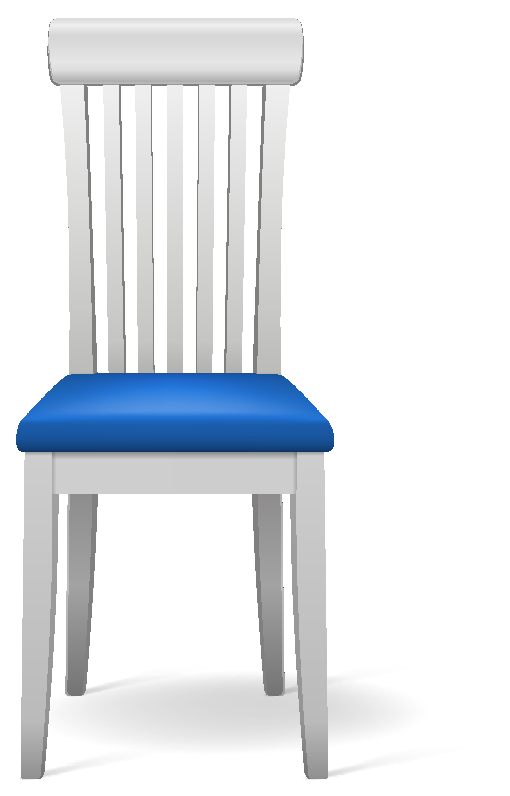
\includegraphics[height=1em]{chair/file.eps}}}$) \quad
  Tim Sherwood \quad
  Rich Wolski
}
\titlegraphic{\hfill\includegraphics[width=2.25cm]{ucsbseal_cmyk.pdf}}

\begin{document}
\maketitle

\metroset{numbering=none}
\begin{frame}<beamer>[noframenumbering]
  \frametitle{Outline}
  \tableofcontents
\end{frame}
\metroset{numbering=fraction}

\section{Motivation}
\begin{frame}{What is a System?}
Infrastructure software upon which applications are built
% (compilers, garbage collectors, file systems, drivers, etc.)
\\
    \vspace{0.2in}
\pause
Operating Systems
  \begin{itemize}[<+->]
      \item Purpose % i.e. they need to be able to do this
          \begin{itemize}
          \item Process abstraction
          \item Named resource management
              \begin{itemize}
                  \item Multiplex physical hardware resources
                  \item Partition and abstract \textbf{memory}
              \end{itemize}
          \end{itemize}
      \item Goals: low overhead, robustness, security
  \end{itemize}
\end{frame}

%\notes{
% isolation third item for os
% files: hide peculiarites of disks/I/O decives, abstract model of device-indepdent files
% address space: virtual memory + protection
% process: running program container (registers, files, alarms, address space, etc.)
%}

\begin{frame}{Systems Languages}
\begin{itemize}[<+->]
    \item Past systems languages: \tiny{ALGOL, PL/I, Fortran, BCPL/B, C, Mesa/Cedar, Pascal/Modula-2/Oberon, C++, ...}
    \item C: the de-facto standard
        \begin{itemize}
            \item Data structure representation control
            \item Memory management control % don't need to use stdlib either
            \item Complete mutability via pointers % define what I mean here
            \item Performant
        \end{itemize}
    \item C: the unsafe standard
        \begin{itemize}
            \item Unchecked array operations $\Rightarrow$ buffer overflows
            \item Pointers $\equiv$ arrays $\Rightarrow$ hazardous pointer arithmetic
            \item Unsafe casts $\Rightarrow$ read/write arbitrary addresses
            \item Aliasing $\Rightarrow$ dangling pointers, double frees, null dereferences
        \end{itemize}
\end{itemize}
\end{frame}

%\notes{
% possibly add OS lang was used for, date
% ALGOL: formally defined syntax
% Mesa, Cedar: rich exceptions, GC
% Pascal (1971), Modula-2 (1982), Oberon (1988) % structured programming, records, pointers, dynamic allocation, information hiding, objects
% see mae3.org, mae4.org
%}

\begin{frame}{Memory Safety}
\begin{itemize}[<+->]
    \item Memory safety error: ``Any dereference of a pointer or subscripted array reference which reads or writes storage outside of the referent'' \footcite{austin_efficient_1994}
        \begin{itemize}
            \item Spatial: outside referent's \alert{address bounds}
            \item Temporal: outside referent's \alert{lifetime}
        \end{itemize}
    \item Ideal technique is
        \begin{itemize}
            \item Efficient and expressive % (hallmarks of C)
            \item Purely static % (no runtime overhead)
            \item Precise % (not overly conservative)
            \item Automatic % (legacy code $\Rightarrow$ no source or memory layout change)
        \end{itemize}
%    \item Non-goals: secrecy, security, concurrency, type safety % but are natural consequences of safety
    \item Memory errors become \alert{type errors}, management happens at \alert{compile-time}
\end{itemize}
\end{frame}

%\notes{
% some of those goals from nagakatte 201*
% undecidability of checking certain dynamic errors
% hard to verify/prove invariants about b/c
  % casts + pointers make c essentially untyped (rondon: type system is only to help know size of bytes to read/write)
  % aliasing
% make bad hard, useful easy
%}

\AtBeginSection[]
{
  \metroset{numbering=none}
  \begin{frame}<beamer>[noframenumbering]
    \frametitle{Outline}
    \tableofcontents[currentsection]
  \end{frame}
  \metroset{numbering=fraction}
}

\only<handout>{
  \addtocounter{framenumber}{1}
}

\section{Spatial Safety}

\begin{frame}[fragile]{Definition and Example}
  \footnotesize
  \begin{columns}[T]
    \begin{column}{0.45\textwidth}
        Prevent accessing out of bounds given to object
        \\
        Some approaches:
        \begin{itemize}
            \item Dynamic \small{(fat pointers, bounds tables, objects)}
            \item Semi-static \small{(via annotations and dependent types})
        \end{itemize}
    \end{column}
    \begin{column}{0.45\textwidth}
%      \lstinputlisting[language=C,mathescape]{lst/spatial_plain.c}
       \begin{lstlisting}[language=C,numbers=left,mathescape,basicstyle={\footnotesize\ttfamily}]
int main() {
    printf("hello, world!\n");
}
$$
        \end{lstlisting}
    \end{column}
  \end{columns}
\end{frame}

\subsection{Some Dynamic Approaches}

\begin{frame}[fragile]{Fat Pointers}
  \footnotesize
A fat pointer structure is contains metadata such as base address and size along with normal value
\\
+ No cost to find metadata
\\
- Incompatible with legacy code
\todo{show example figure in memory}
\end{frame}

\begin{frame}{Fat Pointers}
SafeC \footcite{austin_efficient_1994}:
  \begin{itemize}
     \item Compile-time transform, replace all pointers and extend all pointer definitions
     \item Fields include:
          \begin{itemize}
             \item base, size, storage class (errant deallocations)
             \item Unique capability issued to an allocation
          \end{itemize}
     \item Insert array access checks before each pointer/array dereference
     \item Complete spatial safety as long as
         \begin{itemize}
            \item transparent storage management
            \item no safe pointer object attribute manipulation
         \end{itemize}
     \item 275\% space overhead, 2-6x runtime overhead, 0.35-3x code size overhead
         \begin{itemize}
            \item safe pointers aren't register allocated
            \item compiler optimizations fail with additonal checks
         \end{itemize}
  \end{itemize}
\end{frame}
\begin{frame}{Fat Pointers}
Cyclone \footcite{jim_cyclone_2002}:
  \begin{itemize}
      \item Created with intended target of TAL
      \item Distinguish array pointers from non-array poitners
          \begin{itemize}
             \item never-null pointer
             \item fat pointer
             \item static analysis to warn of uninitialized poitners
           \end{itemize}
      \item Statically validate and remove non-array fat pointers
      \item 40\% runtime overhead
      \item Uses regions + automatic memory management for temporal safety
  \end{itemize}
CCured \footcite{necula_ccured:_2002}:
  \begin{itemize}
      \item Whole-program type inference to statically optimize different pointer uses via a strong type system
        \begin{itemize}
            \item SAFE: almost no overhead, no ptr arith, array indexing, type casts
            \item SEQ: fat pointers allow arith, indexing, some casts
            \item WILD: arbitrary casts, expensive dynamic checks
        \end{itemize}
    \item insert run-time checks to handle portions where static verification insufficient
    \item 3\%-87\% runtime overhead increase
  \end{itemize}
Cuckoo \footcite{west_cuckoo:_2005}
  \begin{itemize}
      \item Store array size in memory before array dimensions's first elem
      \item Check at runtime (compile-time if possible)
      \item Type system for preventing assignment of automatic objects into longer-lifetime pointers
  \end{itemize}
\end{frame}

\begin{frame}[fragile]{Fat Pointers}
       \begin{lstlisting}[language=C,numbers=left,mathescape,basicstyle={\footnotesize\ttfamily}]
int main() {
    printf("hello, world!\n");
}
$$
        \end{lstlisting}
\end{frame}

%% - fullcite:akritidis_baggy_2009
%% - fullcite:brunink_boundless_2011

\begin{frame}[fragile]{Separate Metadata}
Overview: avoid fat pointers by spltting bounds and base metadata
\\
\todo{show example figure in memory}
\\
MSCC \footcite{xu_efficient_2004}
    \begin{itemize}
        \item Shadow structures mirror entire original structure
        \item Checked pointers modified by external libraries must have metadata updated at the library call via wappers
        \item 1.63x overhead
    \end{itemize}
\end{frame}

\begin{frame}{Separate Metadata}
CCured (2005) \footcite{necula_ccured:_2005}
    \begin{itemize}
        \item Improve original CCured work
        \item Reduce number of WILD pointers
            \begin{itemize}
                \item use physical subtyping for handling upcasts
                \item special pointer carrying runtime-type info for downcasts
            \end{itemize}
        \item fix compat issues
            \begin{itemize}
                \item specify conversions, checking at boundaries with precompiled libraries
                \item separate metadata in mirror data structure (perf hit b/c of loss of locality
            \end{itemize}
    \end{itemize}
Softbound \footcite{nagarakatte_softbound:_2009}
    \begin{itemize}
        \item {insert runtime bounds checks, consulting disjoint metadata via table lookup}
        \item {fix disjoint shadow data structure by ...}
        \item handles arbitrary casts, sub-object overflows not covered by MSCC
    \end{itemize}
\end{frame}

\begin{frame}{Separate Metadata}
Checked C \footcite{ruef_checked_2017}
    \begin{itemize}
        \item extend C with two \emph{checked pointer types}
        \item \todo{add back in two items}
%        \item "_Ptr<T>~", a pointer for dereference only (no arith)
%        \item "~_Array_ptr<T>~" and "~_Nt_array_ptr<T>_~", supporting arith w/ bounds declarations in type (latter is ~NUL~ terminated)
        \item isolate (un)safe code with /checked code regions/ at file/func/block level; prevent unchecked pointer usage and certain casts
        \item cannot blame checked code for violation
        \item compiler confirms restrictions maintained, inserts checks (poss optim away) on ptr access
        \item tool to automatically rewrite code to use checked ptrs when possible
    \end{itemize}
\end{frame}

\begin{frame}[fragile]{Separate Metadata}
       \begin{lstlisting}[language=C,numbers=left,mathescape,basicstyle={\footnotesize\ttfamily}]
int main() {
    printf("hello, world!\n");
}
$$
        \end{lstlisting}
\end{frame}

\begin{frame}[fragile]{Separate Metadata}
  \footnotesize
  \begin{columns}[T]
    \begin{column}{0.45\textwidth}
        Foo bar baz
    \end{column}
    \begin{column}{0.45\textwidth}
%      \lstinputlisting[language=C,mathescape]{lst/spatial_objs.c}
       \begin{lstlisting}[language=C,numbers=left,mathescape,basicstyle={\footnotesize\ttfamily}]
int main() {
    printf("hello, world!\n");
}
$$
        \end{lstlisting}
    \end{column}
  \end{columns}
\end{frame}

\subsection{Some Static Approaches}

\subsubsection{Annotations}

\begin{frame}[fragile]{Extended Type Checking}
Extended Type Checking (ETC) \footcite{detlefs_overview_1995}
    \begin{itemize}
      \item use automatic theorem prover to detect index bounds in Modula-3
      \item use info in annotations to assist
      \item easier than C b/c no ptr arithmetic
    \end{itemize}
Also ETC/Java \footcite{flanagan_extended_2002}
\end{frame}

\begin{frame}[fragile]{LCLint}
LCLint \footcite{larochelle_statically_2001}
\begin{itemize}
    \item leverage LCLint, an annotation-assisted *lightweight* detection tool, to detect buffer overflows
    \item more expressive annotations that constrain possible values a reference contains before/after funcall
    \item state func pre/post-cond with ~requires~ and ~ensures~ clauses (prev. also has ~unique~, ~returned~, ~modifies~, ~out~)
    \item assumptions are ~minSet~, ~maxSet~, ~minRead~, ~maxRead~
    \item gives decent examples of use
    \item constraint grammar, LCLint generates constraints at expr level, resolved w/ checking at statement level
    \item heuristics to deal with loops nicely enough
    \item neither sound nor complete
\end{itemize}
\end{frame}

\begin{frame}[fragile]{CSSV}
CSSV \footcite{dor_cssv:_2003}
\begin{itemize}
    \item source-to-source translation
    \item instruments program w/ additional variables describing string attrs
    \item adds ~assert~ statements checking for unsafe string ops
    \item statically analyze instr. version with *integer analysis* to determine possible assertion failures
    \item handles overlapping ptrs, etc.
    \item  disadv: \# vars in instr. quadratic in \# in orig.
\end{itemize}
\end{frame}

%- fullcite:bodik_abcd:_2002 <----
%- fullcite:wagner_first_2000 
%- disadv: proves correct fraction of array/ptr references (useful for reducing checks)

\begin{frame}[fragile]{Annotations Example}
  \footnotesize
       \begin{lstlisting}[language=C,numbers=left,mathescape,basicstyle={\footnotesize\ttfamily}]
int main() {
    printf("hello, world!\n");
}
$$
        \end{lstlisting}
\end{frame}

\subsubsection{Dependent Types}

\begin{frame}{A Quick Look at Syntax, Semantics, and Types}
    Foo
\end{frame}

\begin{frame}{Dependent Types}
    Bar
\end{frame}

% \subsection{Other/Hardware-Support}

\subsection{In Review}

%\begin{frame}{An Overview of Spatial Safety Approaches}
%Several deficiencies
%\begin{itemize}
%  \item High runtime overhead
%  \item Incomplete detection of spatial violations
%  \item Incompatible pointer representations (changing memory layout)
%  \item  Non-trivial changes to source code
%  \item Whole program analyses (for low-overhead) [e.g. Dhurjati 2006, Necula 2005]
%  \item Some of these aren't complete or sound
%  \item  Completely detecting buffer overflow (i.e. bounds) in general is undecidable!
%\end{itemize}
%\end{frame}


\section{Temporal Safety}

\begin{frame}[fragile]{Definition and Example}
  \footnotesize
  \begin{columns}[T]
    \begin{column}{0.45\textwidth}
        Prevent accessing object that has been previously deallocated
        \\
        Some approaches:
        \begin{itemize}
            \item Effects and regions
            \item Unique pointers and linear types
            \item Ownership and borrowing
        \end{itemize}
    \end{column}
    \begin{column}{0.45\textwidth}
%      \lstinputlisting[language=C,mathescape]{lst/spatial_plain.c}
       \begin{lstlisting}[language=C,numbers=left,mathescape,basicstyle={\footnotesize\ttfamily}]
int main() {
    printf("hello, world!\n");
}
$$
        \end{lstlisting}
    \end{column}
  \end{columns}
\end{frame}

\subsection{Dynamic Approaches}
\begin{frame}{A Comment on Garbage Collection}
    \footcite{boehm_garbage_1988}
    used by ccured (Free is a noop, no double-free, no danlging pointers, heapify escaping objects)
\end{frame}
\begin{frame}{Other Dynamic Approaches}
    \footcite{austin_efficient_1994}
    \footcite{west_cuckoo:_2005}
    % others from Other/(also from section)
\end{frame}

\subsection{Semi-Static Approaches}

\end{document}

%%% Local Variables:
%%% mode: latex
%%% TeX-master: t
%%% TeX-engine: xetex
%%% End:
